\documentclass[10pt, a4paper]{article}

\usepackage[utf8]{inputenc}
\usepackage[english]{babel}
\usepackage[T1]{fontenc}
\usepackage{charter}
\usepackage{amsmath}
\usepackage{amssymb}
\usepackage{hyperref}
\usepackage{graphicx}
\usepackage{enumitem}
\usepackage{url}
\usepackage{multirow}
\usepackage{array}
\usepackage{subcaption}
\usepackage{setspace}
\usepackage{booktabs}
\usepackage[nocompress]{cite}
\usepackage{geometry}
\geometry{top=1.3cm,bottom=1.3cm,left=1.6cm,right=1.5cm}
\usepackage{xcolor}
\usepackage{listings}
\usepackage{float}

\pagestyle{plain}


\lstset{basicstyle=\ttfamily,
  showstringspaces=false,
  commentstyle=\color{red},
  keywordstyle=\color{blue},
  basicstyle=\footnotesize	
  %backgroundcolor=\xcolor{backcolour}
}



\begin{document}

\begin{center}

\textbf{Introduction to Computer Vision -- Project Proposal} \\[0.1cm]

\textbf{RA192617 -- Edgar Rodolfo Quispe Condori} \\[0.1cm]
\textbf{RA192618 -- Darwin Ttito Concha} \\[0.1cm]

Institute of Computing, University of Campinas (UNICAMP) \\
Campinas-SP, Brazil, 13083-852 \\

\vspace{0.5cm}
\textbf{\large{Single image crowd person counting}}
\end{center}

In our project we aim to work over the crowd person counting.This is an interesting problem it has applications in safe monitoring, disaster management, design of public places, intelligence gathering, virtual environment, forensic search, among others. The problem can be defined as follow. given and image find the number of persons that appears, as can be see in figure \ref{fig:scenario} the scenarios are really general  and challenging. We intend to use deep learning approach  for the project, the availability of well known architectures (YOLO, Resnet, GoogleNet) and previous inspirings works ~\cite{wang2015deep}\cite{zhang2016single}\cite{shang2016end} suggest that an approach with transfer learning may be feasible for the problem.

\begin{figure}[h!]
\centering
\begin{subfigure}{0.5\textwidth}
  \centering
  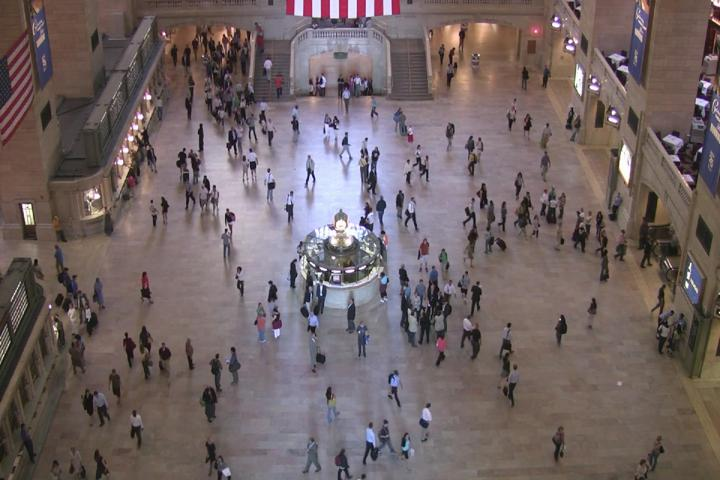
\includegraphics[width=0.9\linewidth]{figs/cover.jpg}
\end{subfigure}%
\begin{subfigure}{0.5\textwidth}
  \centering
  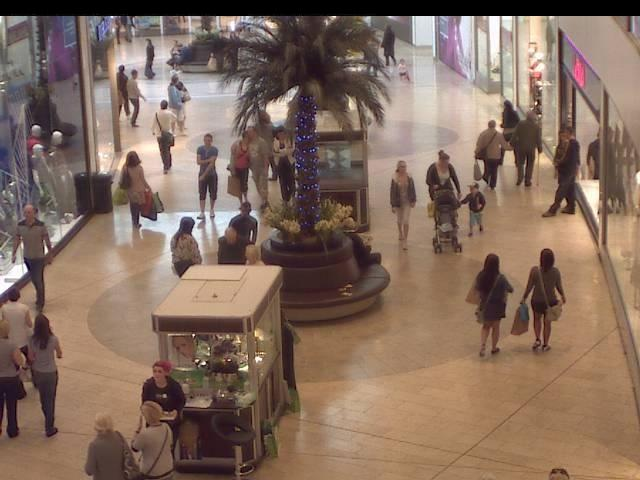
\includegraphics[width=0.8\linewidth]{figs/mallexample.jpg}
\end{subfigure}
  \caption{Examples of inputs for the crowd person counting.}
  \label{fig:scenario}
\end{figure}

In order to test our method we will use the datasets available for the problem, a technical resumo is shown in table \ref{table:datasets}

\begin{table}[H]
\centering
\begin{tabular}{|l|c|c|r|r|r|r|}
\hline
\multicolumn{1}{|c|}{\textbf{Dataset}} & \textbf{Nro. of images} & \textbf{Resolution} & \multicolumn{1}{c|}{\textbf{Min}} & \multicolumn{1}{c|}{\textbf{Ave}} & \multicolumn{1}{c|}{\textbf{Max}} & \multicolumn{1}{c|}{\textbf{Total count}} \\ \hline
\textbf{UCSD} & 2000 & 158x238 & 11 & 25 & 46 & 49,885 \\ \hline
\textbf{Mall} & 2000 & 320x240 & 13 & - & 53 & 62, 325 \\ \hline
\textbf{UCF\_CC\_50} & 50 & Varied & 94 & 1279 & 4543 & 63,974 \\ \hline
\textbf{WorldExpo'10} & 3980 & 576x720 & 1 & 50 & 253 & 199,923 \\ \hline
\textbf{ShanghaiTech Part A} & 482 & Varied & 33 & 501 & 3139 & 241,677 \\ \hline
\textbf{ShanghaiTech Part B} & 716 & 768 x 1024 & 9 & 123 & 578 & 88,488 \\ \hline
\end{tabular}
\caption{Available datasets for crowd person couting.}
\label{table:datasets}
\end{table}

\bibliographystyle{unsrt}
\bibliography{proposal}

\end{document}
